%% Beispiel f�r Klasse tudposter.cls (Version 0.5).
%%
%% Autor: Martin Zabel (martin.zabel@tu-dresden.de)
%%
%% Klassenoptionen siehe tudposter.cls.
%%
%% Wir bevorzugen PDFLaTeX. F�r den Fall, dass die CD-Schriften nicht
%% in der Standardkonfiguration erw�hnt sind laden wir die .map-Datei
%% Wichtig: das muss vor dem ersten Font-Befehl (also vor der
%% Dokumentklasse geschehen.
\pdfmapfile{+univers.map}
%%
\documentclass[a0paper,noDIN,Mathematik]{tudmathposter}

% Bei Bedarf: dinBold f�r Section. Dann aber auch �berschrift nur in
% Gro�buchstaben.
%\addtokomafont{section}{\dinBold}

% In diesem Poster ben�tigte Pakete.
% Jedem wie es beliebt.
\usepackage[T1]{fontenc}
\usepackage[latin1]{inputenc} % latin1 (Linux) oder ansinew (Win) wenn
                            % nicht UTF 8
\usepackage[ngerman]{babel}
\usepackage{multicol}
\usepackage{tikz}
\usepackage{amsmath}
\usepackage{lipsum}
\usepackage{amsthm}
\usepackage{subfig}                % for subfigures
\usepackage{wrapfig}               % for in-text figures
\usepackage{listings}              % for source-codes
\usepackage{url}

% Beschriftung im Seitenkopf und Seitenfu�
%\einrichtung{Fakult�t f�r Mathematik und Informatik}
\institut{Institut f�r Algebra}
\professur{Professur f�r \TeX nische Algebra}
\author{Mike Behrisch}% Zum Beispiel f�r Kontaktdaten.
\telefon{0351 463-34224}
\fax{0351 463-34235}
\homepage{http://www.math.tu-dresden.de/\textasciitilde mbehri/}


\title{Evaluation der FR Mathematik}
\subtitle{Ein Beispielposter}

\newtheorem{definition}{Definition}
\begin{document}
%\color{HKS41K100}%
%%%%%%%%%%%%%%%%%%%%%%%%%%%%%%%%%%%%%%%%%%%%%%%%%%%%%%%%%%%%%%%%%%%%%%%%%%%%
%%% Poster-Titel
%%%%%%%%%%%%%%%%%%%%%%%%%%%%%%%%%%%%%%%%%%%%%%%%%%%%%%%%%%%%%%%%%%%%%%%%%%%%
\maketitle
%%%%%%%%%%%%%%%%%%%%%%%%%%%%%%%%%%%%%%%%%%%%%%%%%%%%%%%%%%%%%%%%%%%%%%%%%%%%
%%% Poster-Inhalt
%%%
%%% Hinweis:
%%%   \raggedright muss nach jedem Kommando aufgerufen, dass die
%%%   Absatzformatierung wieder zur�ckstellt. Beispiele:
%%%   \begin{minipage}, \parbox.
%%% 
%%%%%%%%%%%%%%%%%%%%%%%%%%%%%%%%%%%%%%%%%%%%%%%%%%%%%%%%%%%%%%%%%%%%%%%%%%%%
%\raggedright%Linksb�ndig
% Zur Abwechselung mal ein dreispaltiges Layout.
\setlength{\columnsep}{1.5cm}%
\setlength{\multicolsep}{0pt}%

\section{Die Einleitung (einmal mehrspaltig)}
\begin{multicols}{3}%
\lipsum[1]
\end{multicols}\vspace{3ex}

\section{Die Definition}
\begin{minipage}{0.7\textwidth}
  \begin{definition}
    Wir nennen einen Verband $\mathbf{L}$ \emph{verbandelt}, wenn seine Kardinalit�t eine Schnapszahl ist. Dies wird durch folgende Gleichung symbolisiert:
    \[\lim_{\infty \to 3}\sqrt{2 + |\mathbf{L}|} = 5.\]
  \end{definition}
  Die nebenstehende Abbildung zeigt einen verbandelten Verband.\par

 Die Text-Bild-Aufteilung wurde durch zwei nebeneinandeplazierte \texttt{minipages} erreicht. Hierbei ist der Nachteil, da� das Bild nicht in eine \texttt{figure}-Umgebung eingebunden werden kann. Dies ist aber bei einem Poster  ohnehin nicht sehr sinnvoll, da Abbildungen meist fixiert und nicht beweglich sein sollten.
\end{minipage}
\begin{minipage}{0.3\textwidth}
  \centering
  \includegraphics*[keepaspectratio,width=0.3\textwidth,height=3cm,angle=30]{image2}
\end{minipage}\vspace{3ex}

\section{Ein Bild im Text}
\begin{multicols}{2}
Mathematik macht Spa�, besonders, wenn ein Bild dabei ist. Solche Bilder sind normalerweise immer an einer Extrastelle au�erhalb des Textes.   \begin{wrapfigure}{l}{0.3\textwidth}
    \begin{center}
      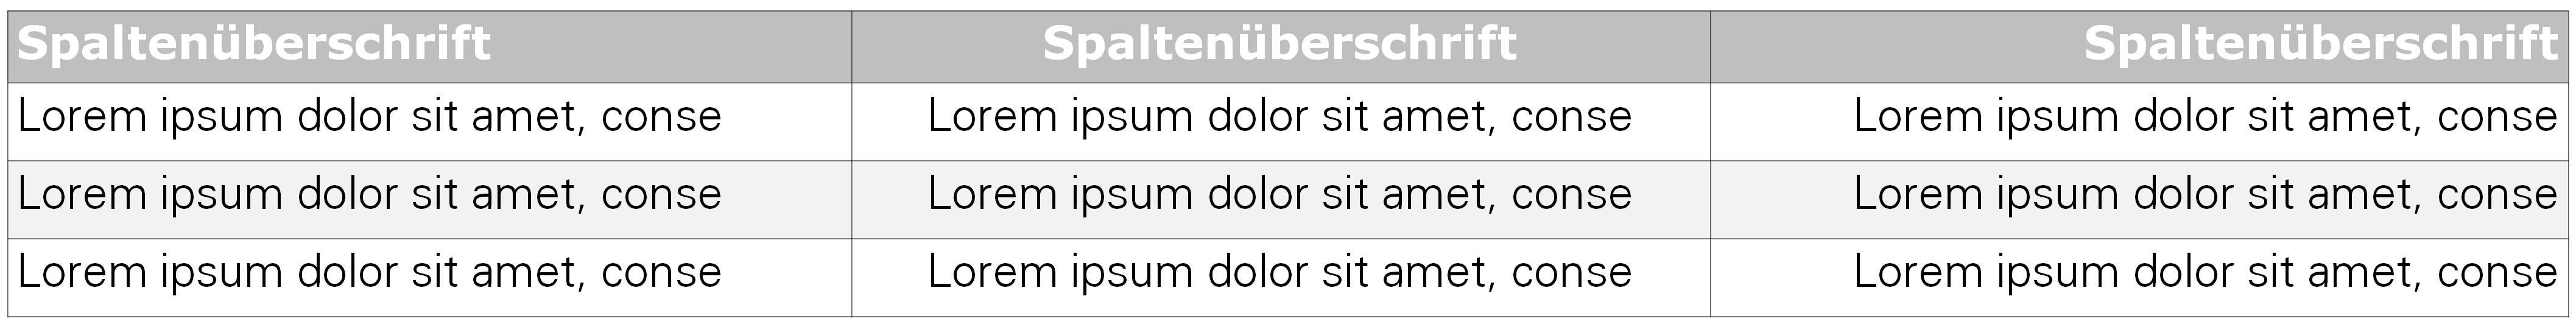
\includegraphics[width=0.28\textwidth]{image1}
    \end{center}
    \caption{Bild}
  \end{wrapfigure}
Wenn man das Paket \verb+wrapfig+ einbindet, dann l��t sich eine Graphik auch rechts vom Text umflie�en oder links vom Text umflie�en. Die Graphik wird dazu einfach in \verb+\begin{wrapfigure}{Seite}{Breite}+ und \verb+\end{wrapfigure}+ eingeschlossen. Dabei kann \verb+Seite+ die Werte  \texttt{l} 
f�r ``links'' und \texttt{r} f�r ``rechts'' annehmen und bezeichnet die Position der Graphik relativ zum umflie�enden Text. Der Parameter \texttt{Breite} gibt die Breite der Graphik an.\par 

Hinweis: Es kann sinnvoll sein, innerhalb der \texttt{wrapfigure}-Umgebung den Befehl \verb+\vspace{VertikalerAbstand}+ mit einem negativen Wert f�r 
\texttt{VertikalerAbstand} zu verwenden.
\end{multicols}

\section{Mehrere Bilder zusammen}

Man kann auch mehrere graphische Darstellungen in einer Abbildungumgebung zusammenfassen. Das zugeh�rige Paket hei�t \verb+subfig+, der notwendige Befehl in der \texttt{figure}-Umgebung hei�t \verb+\subfloat[Bildunterschrift]{Bildeinbindungsbefehl}+, etwa
\begin{verbatim}
\subfloat[A picture]{\label{fig:image41}
\includegraphics[width=0.3\textwidth]{image4}}
\end{verbatim}
Das Ergebnis ist in Abbildung~\ref{fig:severalthings} zu sehen.%
\begin{figure*}[h!]
  \centering
  \subfloat[A picture]{\label{fig:image41}
\includegraphics[width=0.3\textwidth]{image4}}                
  \subfloat[A slightly rotated picture]{\label{fig:image42}
\includegraphics[keepaspectratio,angle=45,width=0.3\textwidth]{image4}}
  \subfloat[A rather rotated picture]{\label{fig:image43}
\includegraphics[keepaspectratio,angle=125,width=0.3\textwidth]{image4}}
  \caption{Several things in one figure}
  \label{fig:severalthings}
\end{figure*}

\section{Manchmal will man auch einen Quelltext einbinden\ldots}
\begin{minipage}[t]{0.55\textwidth}
Das geht mit dem Paket \texttt{listings}. Die einfachste Variante ist seinen Programmcode einfach in \verb+\begin{lstlisting}+ und \verb+\end{lstlisting}+ einzuschachteln. Wenn das Programm l�nger ist kann man auch einfach eine Quelldatei mit \verb+\lstinputlisting[language=proglang]{source_filename.yourlanguage}+ direkt einbinden. Dabei wird dann eine automatische Quelltexthervorhebung in Abh�ngigkeit der durch den Wert \texttt{proglang} gew�hlten Programmiersprache durchgef�hrt.
\end{minipage}\hspace{0.05\textwidth}
\begin{minipage}[t]{0.4\textwidth}
\begin{lstlisting}[language=C++]
#include <iostream>
using namespace std;

int main()
{
   cout << "Hello World" << endl;
   return 0;
}
\end{lstlisting}
\end{minipage}

\section{Bilder selbst entwerfen}

Wenn man gezwungen ist, mal eine Abbildung selbst zu entwerfen, so empfehlen wir das Paket \texttt{tikz}. Dessen Syntax ist relativ einfach zu erlernen, und dennoch besitzt dieses Paket relativ umfassende M�glichkeiten. Im Internet sind unter \url{http://www.texample.net/tikz/examples/} zu finden.
%  Es wird hier ein sehr einfaches und ein etwas komplizierteres Beispiel mitgeliefert. Viele weitere Beispiele sind im Internet unter \url{http://www.texample.net/tikz/examples/} zu finden.

% \begin{tikzpicture}[%text height=1.5ex,text depth=.35ex,
%                     latnode/.style={thick,circle,draw=black,inner sep=0mm,minimum size = 3mm}]
%   \node[latnode, label=below:$0$  ]    (0)   at ( 0,0) {};
%   \node[latnode, label=right:$z$  ]    (z)   at ( 0,1) {};
%   \node[latnode, label=above:$y$  ]    (y)   at ( 0,2) {};
%   \node[latnode, label=left :$a_1$]    (a)   at (-2,2) {};
%   \node[latnode, label=left :$b_1$]    (b)   at (-2,4) {};
%   \node[latnode, label=right:$a_2$]    (A)   at ( 2,2) {};
%   \node[latnode, label=right:$b_2$]    (B)   at ( 2,4) {};
%   \node[latnode                   ]    (avA) at ( 0,4) {};
%   \node[latnode, label=above:$1$  ]    (1)   at ( 0,6) {};
%   \draw[-] (0)   -- (z);
%   \draw[-] (z)   -- (y);
%   \draw[-] (0)   -- (a);
%   \draw[-] (0)   -- (A);
%   \draw[-] (a)   -- (b);
%   \draw[-] (A)   -- (B);
%   \draw[-] (a)   -- (avA);
%   \draw[-] (A)   -- (avA);
%   \draw[-] (b)   -- (1);
%   \draw[-] (B)   -- (1);
%   \draw[-] (avA) -- (1);
%   \draw[-] (y)   -- (b);
%   \draw[-] (y)   -- (B);
% \end{tikzpicture}


\end{document}
%-----------------------------------------------------------------------------------
\pagebreak
\title{2. Plakat}%
\subtitle{testausgaben}%
\maketitle
\section*{Test Aufz�hlung}
\begin{multicols}{2}
Dies ist eine Aufz�hlung.

\begin{itemize}
\item Item
\item Item
  \begin{itemize}
  \item SubItem
  \item SubItem
  \item SubItem
  \end{itemize}
\item Item
\item Item
\item Item
\item Item
\item Item
\item[\raisebox{.2ex}{$\Rightarrow$}] Ergebnis
\end{itemize}

\section*{Test Buchstaben / Zahlen}
A B C D E F G H I J K L M N O P Q R S T U V W X Y Z � � �.
a b c d e f g h i j k l m n o p q r s t u v w x y z � � � �.
0 1 2 3 4 5 6 7 8 9.

\section*{Test Unterabschnitte}
\subsection*{Unterabschnitt 1}
Dies ist ein Absatz.
\subsection*{Unterabschnitt 2}
Dies ist ein noch ein Absatz.

\vfill
%\columnbreak
\section*{Test Mathematisches}
Vergleich Schriftart in Text und Formel:\\
1+2=3 vs. $1+2=3$.

Abgesetze Formeln:
\begin{eqnarray}
\mbox{Gleichung:}&&1+2*3-4/5\approx6\\
\mbox{Funktion:}&&A(r)=\pi r^2\\
\mbox{Funktionsnamen:}&&\lim_{n\to0}\frac{1}{n}=\infty\\
\mbox{Summensymbol:}&&e=\sum_{k=0}^{\infty}\frac{1}{k!}\\
\end{eqnarray}

\vfill
%\columnbreak
\section*{Test Grafik}
\rule{\linewidth}{2cm}
\end{multicols}

\begin{multicols}{2}
\makeatletter
\@tempdima=1cm
1cm = $\the\@tempdima$\\
\makeatother
topmargin = $\the\topmargin$\\
headheight = $\the\headheight$\\
headsep = $\the\headsep$\\
topskip = $\the\topskip$\\
baselineskip = $\the\baselineskip$\\
footskip = $\the\footskip$\\
{\textcolor{black}{
textheight = $\the\textheight$}}\\
oddsidemargin = $\the\oddsidemargin$\\
evensidemargin = $\the\evensidemargin$\\
textwidth = $\the\textwidth$\\
paperheight = $\the\paperheight$\\
paperwidth = $\the\paperwidth$
\end{multicols}
\iffalse
%\definecolor{mathelogoblau}{cmyk}{0.96,0.7,0.00,0.07}
%\definecolor{mathelogorot}{cmyk}{0.00,0.99,0.95,0.00}
%\definecolor{mathelogoviolett}{cmyk}{0.27,0.99,0.00,0.03}
% das sollte man nicht machen, da f�r den Druck cmyk gebraucht wird
% aber ich habe nur RGB
\definecolor{mathelogoblau}{rgb}{0.0392,0.2784,0.9294}
\definecolor{mathelogorot}{rgb}{1,0.0117,0.051}
\definecolor{mathelogoviolett}{rgb}{0.7098,0.0117,0.9686}

\begin{tikzpicture}[scale=4]
\fill [mathelogoviolett] (0,0) rectangle (1,-1);
\fill [mathelogoblau,rotate=36.8] (0,0) rectangle (0.8,0.8);
\fill [mathelogorot,rotate around={-53:(1,0)}] (0.4,0) rectangle (1,0.6);
\end{tikzpicture}
\fi
\vfill
Diese Hilfslinie zeigt das Seitenende an. \textbf{ZU ENTFERNEN}!
\hrule
\end{document}
